\phantomsection\numberedsection{RF6.4 Borrar Atributo}

\subsection*{Descripción}
Los usuarios pueden borrar los atributos de usuario ya existentes en la cuenta.
\vspace{0.15cm}

\textbf{Pre-condición}\par
El usuario ha iniciado sesión en su cuenta en Mini PIM y hay al menos un atributo de usuario creado.\par
\vspace{0.15cm}

\textbf{Post-condición}
\begin{itemize}
    \item Caso de éxito: El atributo es borrado y eliminado de la base de datos.
    \item Caso mínimo: El sistema notifica al usuario el resultado de la acción borrar atributo; exitosa o fallida.
\end{itemize}

\textbf{Prioridad: }
Alta
\vspace{0.15cm}

\textbf{Autor: }
Diego Sicre y Francisco Javier Jordá Garay\par
\vspace{0.15cm}

\textbf{Control de cambios: }
\begin{itemize}
    \item Versión 1: Definición del caso de uso.
\end{itemize}


\numberedsubsection{Escenario principal}
\begin{enumerate}
    \item El usuario selecciona el atributo que quiere borrar.
    \item El usuario pulsa el opción de \enquote{Borrar}.
    \item El sistema pregunta al usuario si está seguro de su decisión.
    \item El usuario confirma seleccionando \enquote{Sí}.
    \item El sistema borra el atributo de la base de datos.
    \item El sistema muestra al usuario un mensaje confirmando que el atributo ha sido borrado con éxito.
\end{enumerate}

\numberedsubsection{Escenarios alternativos}
\begin{description}

    \item[4.a] El usuario decide no borrar el atributo.
    \begin{enumerate}
        \item[4.a.1] El usuario selecciona \enquote{No} en el mensaje de confirmación.
        \item[4.a.2] El sistema cancela la acción de borrado.
        \item[4.a.3] El sistema muestra la lista de atributos sin cambios.  
    \end{enumerate}
    \item[4.b] El usuario decide borrar el atributo pero está ligado a algún(os) producto(s).
    \begin{enumerate}
        \item[4.b.1] El usuario selecciona \enquote{Si} en el mensaje de confirmación.
        \item[4.b.2] El sistema notifica al usuario de que existen productos asociados al atributo que se desea borrar.
        \item[4.b.3] El sistema muestra un listado de los productos asociados al atributo.
        \item[4.b.4] El sistema pregunta al usuario si realmente quiere borrar el atributo.
        \begin{enumerate}
            \item[4.b.4.a.1] El usuario selecciona \enquote{No} en el mensaje de confirmación.
            \item[4.b.4.a.2] El sistema cancela la acción de borrado.
            \item[4.b.4.a.3] El sistema muestra la lista de atributos sin cambios 
        \end{enumerate}
        \begin{enumerate}
            \item[4.b.4.b.1] El usuario selecciona \enquote{Si} en el mensaje de confirmación.
            \item[4.b.4.b.2] El sistema borra el atributo. 
            \item[4.b.4.b.3] El sistema actualiza todos los productos relacionados al atributo borrado asignando un valor nulo. 
            \item[4.b.4.b.4] El sistema muestra la lista de atributos sin el atributo borrado.
        \end{enumerate} 
    \end{enumerate}
\end{description}

\numberedsubsection{Casos de Prueba}
\underline{Escenario: Principal}\par
\vspace{0.15cm}
\textbf{Dado} que el usuario ha iniciado sesión en su cuenta en Mini PIM,\par
\textbf{Y} se encuentra en la sección de atributos,\par
\textbf{Y} selecciona un atributo,\par
\textbf{Cuando} pulsa el botón de \enquote{Borrar},\par
\textbf{Y} confirma la acción,\par
\textbf{Entonces} el sistema borra el atributo de la base de datos y vuelve a mostrar la lista de atributos.\par
\vspace{0.20cm}

\underline{Escenario: Alternativo 3.a}\par
\vspace{0.15cm}
\textbf{Dado} que el usuario ha iniciado la acción de \enquote{Borrar} un atributo,\par
\textbf{Y} el sistema muestra un mensaje de confirmación,\par
\textbf{Cuando} el usuario selecciona \enquote{No} en la confirmación,\par
\textbf{Entonces} el sistema cancela la acción,\par
\textbf{Y} muestra la lista de atributos sin cambios.\par

\vspace{0.20cm}

\numberedsubsection{Bocetos}
\begin{figure}[H]
    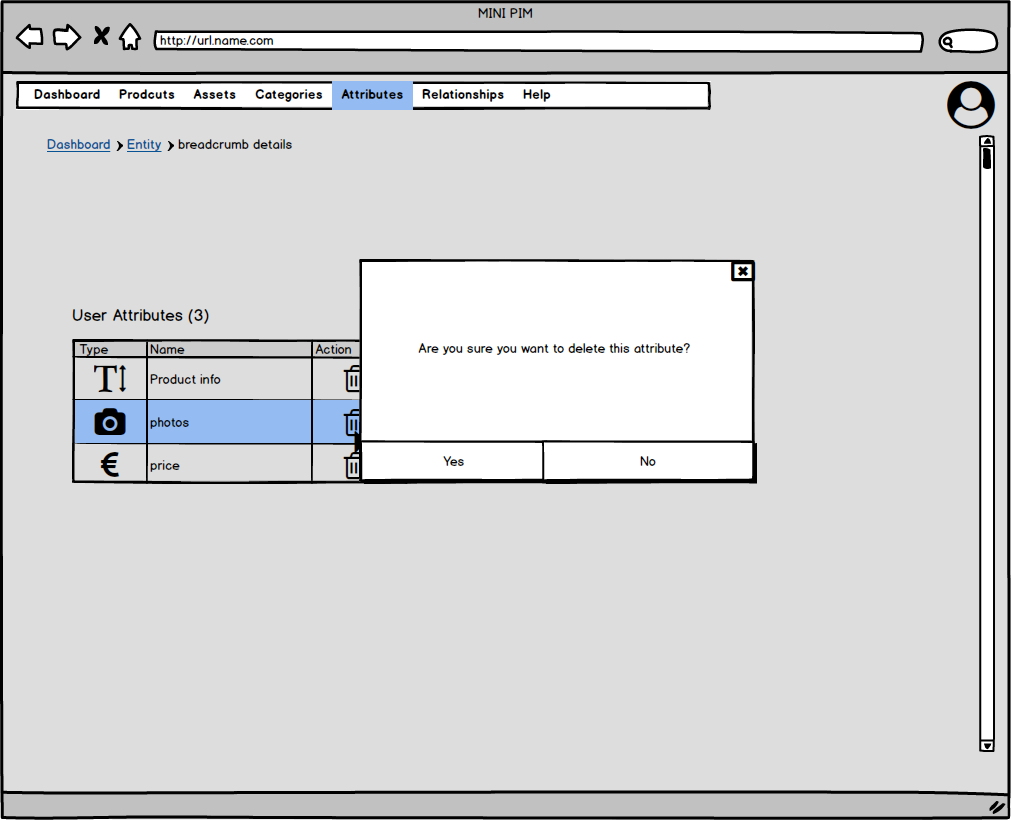
\includegraphics[width=1\linewidth]{mockups/RF6.4BorrarAtributo.png}
    \caption{Apartado Atributos hacer clic en \enquote{Borrar}}
   \end{figure}
\vspace{1.0cm}

\begin{figure}[H]
    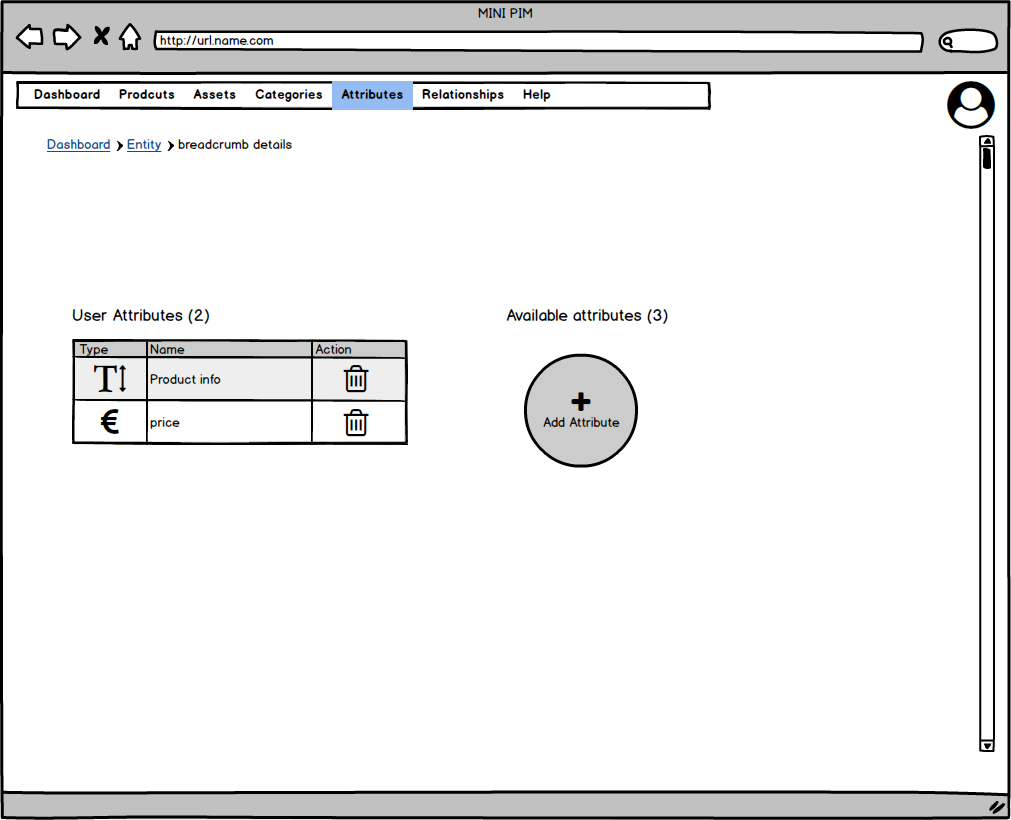
\includegraphics[width=1\linewidth]{mockups/RF6.4BorrarAtributoDespuesDeBorrar.png}
    \caption{Apartado Atributos tras clicar \enquote{Borrar} y confirmar eliminación}
   \end{figure}
\vspace{1.0cm}




\newpage %Inicia en una nueva página otro caso de uso